% -*-  mode: TeX-PDF-mode;  -*-
\documentclass[compress]{beamer}
\mode<presentation>

\usetheme{metropolis}
\graphicspath{{./}{images/}}

\definecolor{darkgreen}{rgb}{0, .6, 0}
\definecolor{darkred}{rgb}{.75,0,0}

% include packages
\usepackage[english]{babel}
\usepackage[utf8]{inputenc}
\usepackage{lmodern}
\usepackage{scalefnt}
\usepackage{attrib}
\usepackage{multicol}
\usepackage{mathtools}
\usepackage[compatibility=false]{caption}
\usepackage{booktabs}
\usepackage{csquotes}
\usepackage{siunitx}
\usepackage{graphicx}
\usepackage{tikz}
\usepackage{standalone}
\usepackage{url}
\usepackage{multimedia}
\usepackage{hyperref}
\usepackage{url}
\usepackage{braket}
\usepackage{verbatim}
\usepackage{tcolorbox}
\usepackage{relsize}
\usepackage{subcaption}
\usepackage{allrunes}
\usepackage{siunitx}
\usepackage{textcomp}
\usepackage[normalem]{ulem}
\usetikzlibrary{shapes.geometric,shapes,positioning,shapes.symbols,arrows,calc,fit,external}

\tcbuselibrary{listingsutf8,breakable,theorems,skins}

\captionsetup[figure]{labelformat=empty}
\captionsetup[table]{labelformat=empty}
\setbeamertemplate{caption}{\insertcaption}

\setbeamertemplate{footline}[text line]{%
%LEO: I need footnotes.%\parbox{\linewidth}{\vspace*{-12pt}\hfill{}JonathanJogenfors\hfill{}\texttt{jonathan.jogenfors@liu.se}\hfill\insertframenumber/\inserttotalframenumber}}
\parbox{\linewidth}{\vspace*{-12pt}\hfill{}\hfill{}\hfill\insertframenumber/\inserttotalframenumber}}
\setbeamertemplate{navigation symbols}{}


\setbeamerfont{subtitle}{series=\normalfont}

\title{Detection fo Attacks}
\subtitle{Securing critical information infrastructures}
\author{Jonathan Jogenfors\\ Leonardo Iwaya}
\date{2016-09-26}

\newtcbinputlisting[]{\listing}[1][]{%
    listing only,
    fontupper=\huge,
}
\begin{document}
\small
\frame{\titlepage}
\begin{frame}{Introduction}
    \begin{columns}
        \begin{column}{0.8\textwidth}
    \begin{itemize}
        \item About us
    \end{itemize}
        \end{column}
        \begin{column}{0.2\textwidth}  %%<--- here
            \begin{center}

                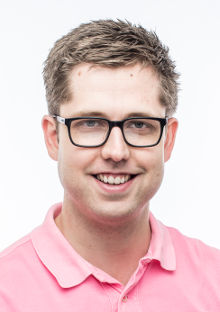
\includegraphics[width=\textwidth]{jonathan.jpg}


            \end{center}
        \end{column}
    \end{columns}
\end{frame}
\begin{frame}
    \begin{itemize}
        \item Model of information security: Prevention, Detection, Reaction
            (PRD)
            \begin{itemize}
                \item Prevention: Difficult because attacker has the advantage.
                    Large attack surface.


                \item
                    Reaction: Too late!
                \item
                    Detection: What our papers are all about
            \end{itemize}
        \item

    \end{itemize}
\end{frame}
\begin{frame}{When prevention fails}

\end{frame}
\begin{frame}{Anomaly detection}

\end{frame}
\begin{frame}{Intrusion Detection Systems \& Honeypots}
\begin{figure}
 \centering
 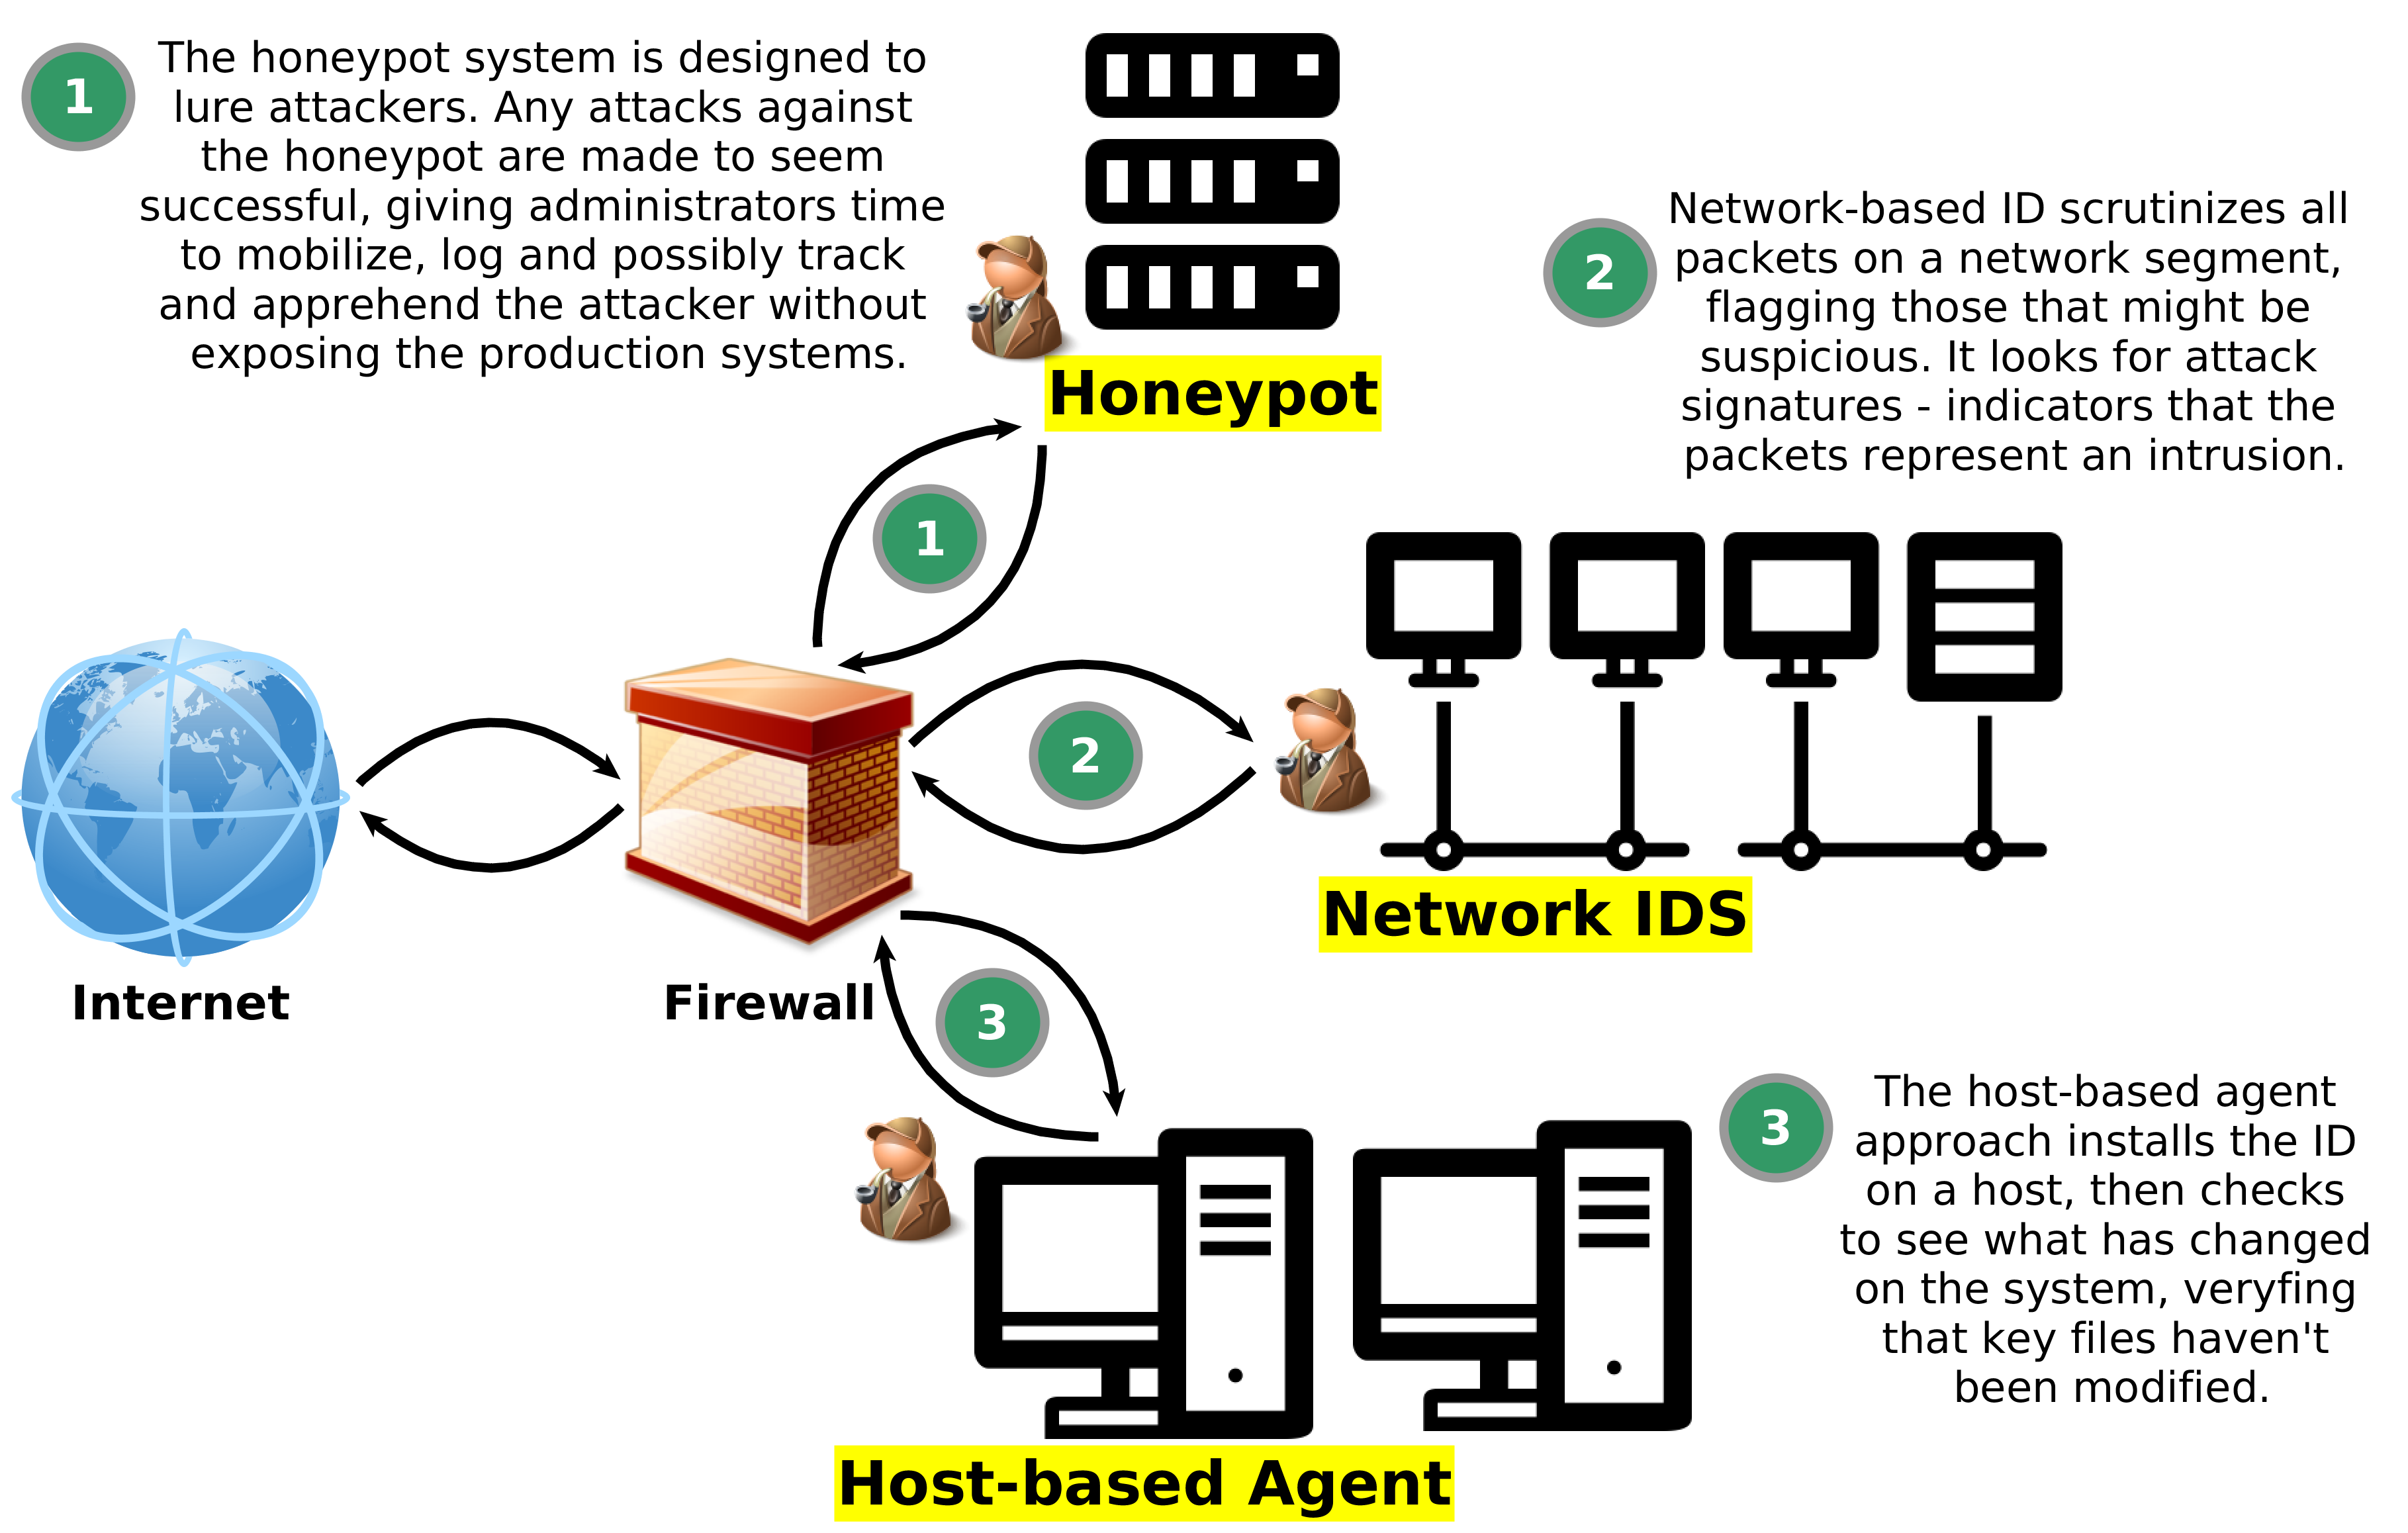
\includegraphics[width=1.0\textwidth]{./images/ids-and-honeypot.png}
 % ids-and-honeypot.png: 0x0 pixel, 300dpi, 0.00x0.00 cm, bb=
 \caption{Source: http://www.computerworld.com/article/2592425/lan-wan/intrusion-detection.html}
 \label{fig:ids-and-honeypot}
\end{figure}

\end{frame}
\begin{frame}{Control Theory \& Cybernetics}
    \textbf{Control systems}: measure, compare, compute and correct.
    \begin{figure}
    \centering\tiny
    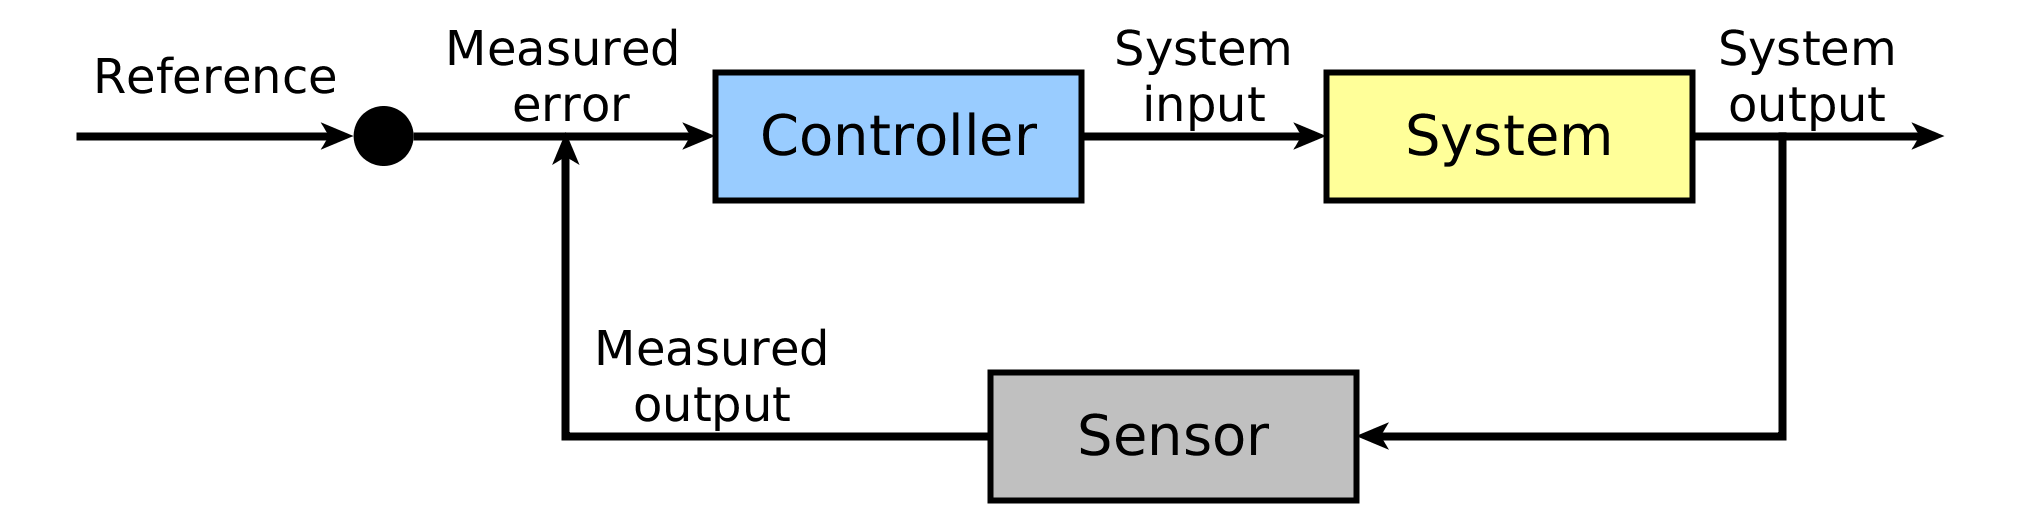
\includegraphics[width=1.0\textwidth]{./images/control-theory.png}
    % control-theory.png: 0x0 pixel, 300dpi, 0.00x0.00 cm, bb=
    \caption{\textbf{Feedback loop} to control the behavior of a system by comparing its output to a desired value, and applying the difference as an error signal to dynamically change the output so it is closer to the desired output.}
    \label{fig:control-theory}
    \end{figure}
\end{frame}
\begin{frame}{Papers}
    \textbf{Motivation}
    \begin{itemize}
     \item Papers \cite{pasqualetti2013attack} and \cite{genge2015system} were \textbf{selected} based on their \textbf{relevance} to the theme of \textit{``attack detection methods''} for \textit{``critical infrastructures''}. 
     \item Paper \cite{vasilo2016multi} was in the course's reading list.

    \end{itemize}
    \begin{table}\tiny
	\begin{tabular}{|l|l|l|l|l|}
	\hline
	\textbf{Paper} & \textbf{Year} & \textbf{CI Sub-area} & \textbf{Citations} & \textbf{Journal IF}\\ 
	\hline \hline
	Pasqualetti et al \cite{pasqualetti2013attack} & 2013 & Attack Detection & 210 & 2.777\\
	Genge et al \cite{genge2015system} & 2015 & Attack Prevention \& Detection & 12 & 1.351\\
	Vasilomanolakis et al \cite{vasilo2016multi} & 2016 & Attack Detection & 1 & n.a \\
	\hline
	\end{tabular}
    \end{table}
\end{frame}
\begin{frame}{Attack detection and identification in cyberphysical systems
    (2013)}

\end{frame}
\begin{frame}{A system dynamics approach for assessing the impact of cyber attacks on CI (2015)}
    \textbf{Aim \& Contribution}
    \begin{itemize}
     \item To \textbf{identify} and \textbf{rank} assets in complex, large-scale and heterogeneous CIs.
     \item \textbf{Cyber Attack Impact Assessment} (CAIA) methodology that helps system admins to understand:
     \begin{enumerate}
      \item How cyber attacks affect the normal functioning of physical processes?
      \item What cyber assets would cause the most negative impact if compromised?
     \end{enumerate}
    \end{itemize}
\end{frame}
\begin{frame}{A system dynamics approach for assessing the impact of cyber attacks on CI (2015)}
    \textbf{CAIA Methodology}
    \begin{figure}
      \centering
      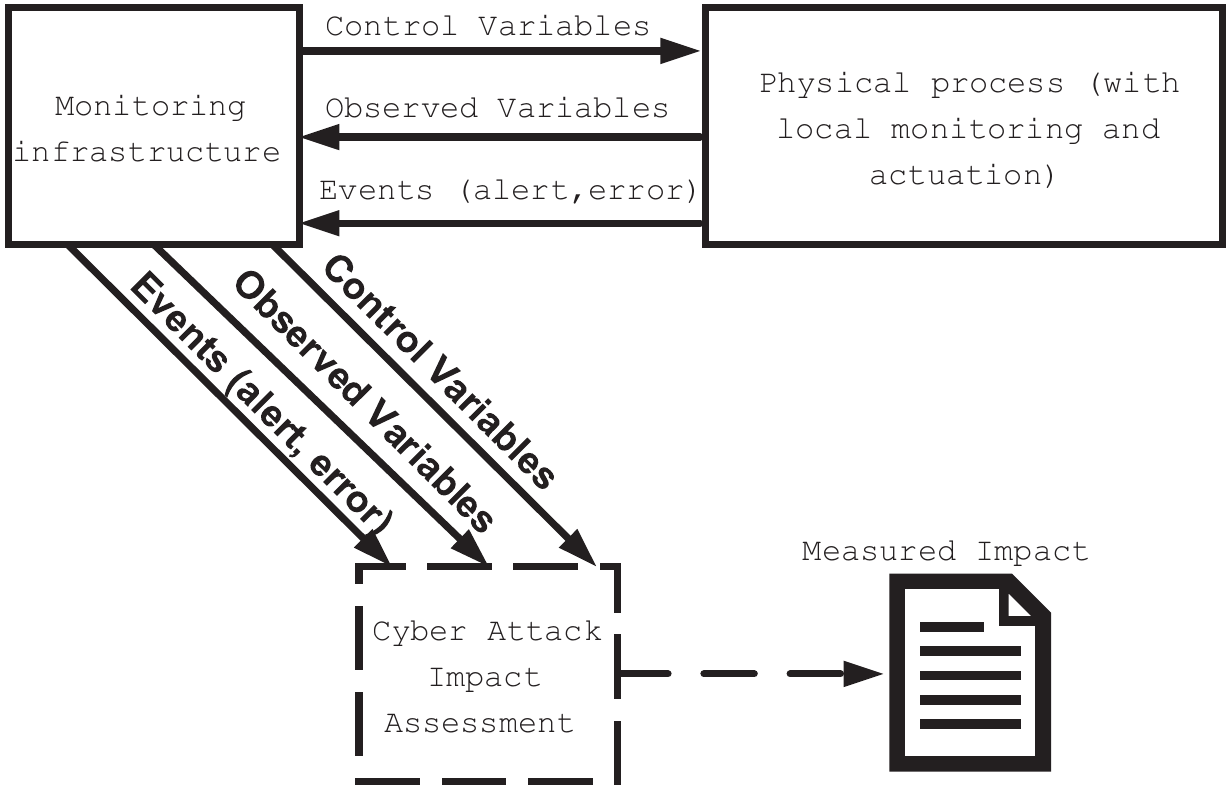
\includegraphics[width = 0.75\textwidth]{./images/caia-method.png}
      % caia-method.jpg: 0x0 pixel, 300dpi, 0.00x0.00 cm, bb=
      % \caption{CAIA Methodology.}
      \label{fig:caia-method}
    \end{figure}
\end{frame}
\begin{frame}{A system dynamics approach for assessing the impact of cyber attacks on CI (2015)}
    \textbf{Experiments \& Comparisons}
    \begin{itemize}
     \item First, the \textbf{basic functioning} of CAIA is demonstrated using IEEE 14-bus electric grid model.
     \item Second, CAIA's \textbf{scalability} is proven by using attack scenarios in the context of IEEE 300-bus electric grid model.
     \item Third, CAIA's \textbf{cross-sector applicability} is evaluated using Tennessee Eastman chemical process system.
     \item The methodology was also \textbf{compared} with other approaches (i.e., graph-theoretic and electrical centrality metric techniques).
    \end{itemize}
\end{frame}
\begin{frame}{A system dynamics approach for assessing the impact of cyber attacks on CI (2015)}
    \begin{columns}
     \begin{column}{0.55\textwidth}
      \begin{figure}
      \centering
      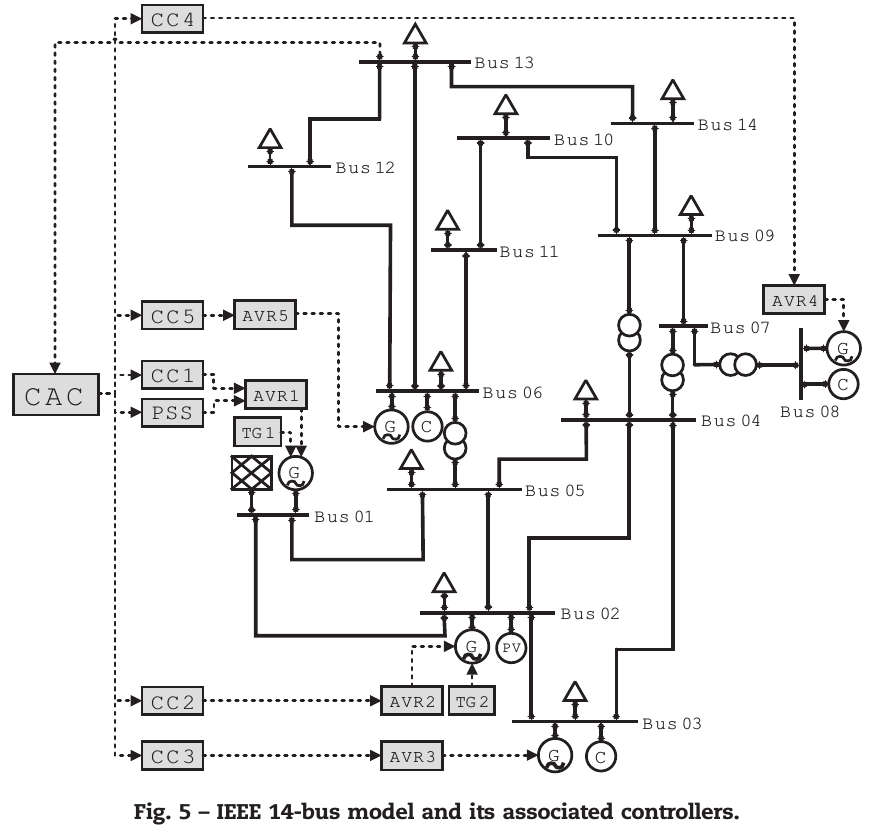
\includegraphics[width=1.0\textwidth]{./images/ieee-14-bus.png}
      % ieee-14-bus.png: 0x0 pixel, 300dpi, 0.00x0.00 cm, bb=
      \label{fig:ieee-14-bus}
      \end{figure}
     \end{column}
     \begin{column}{0.45\textwidth}
      \begin{figure}
      \centering
      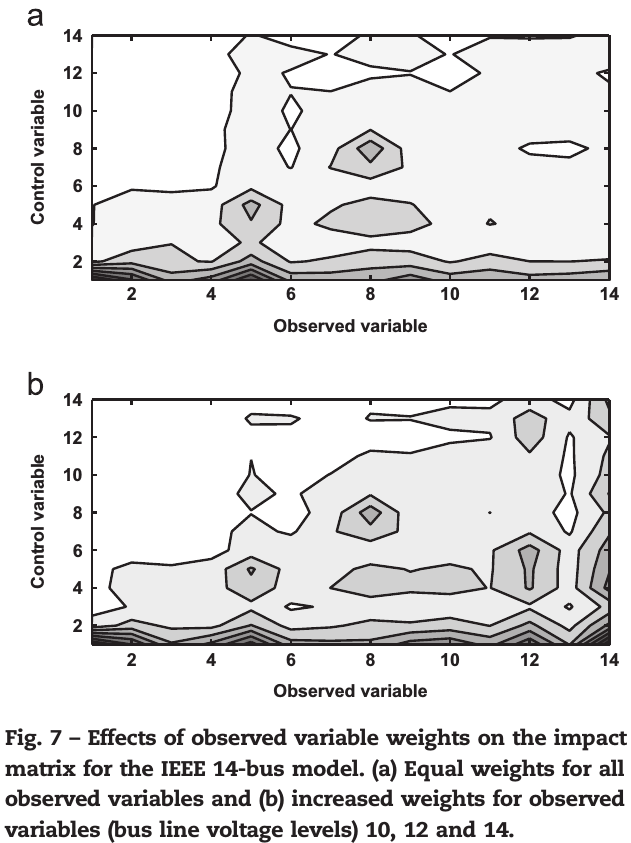
\includegraphics[width=1.0\textwidth]{./images/caia-param.png}
      % caia-param.png: 0x0 pixel, 300dpi, 0.00x0.00 cm, bb=
      \label{fig:caia-param}
      \end{figure}
     \end{column}
    \end{columns}
\end{frame}
\begin{frame}{A system dynamics approach for assessing the impact of cyber attacks on CI (2015)}
    \begin{columns}
     \begin{column}{0.55\textwidth}
      \begin{figure}
      \centering
      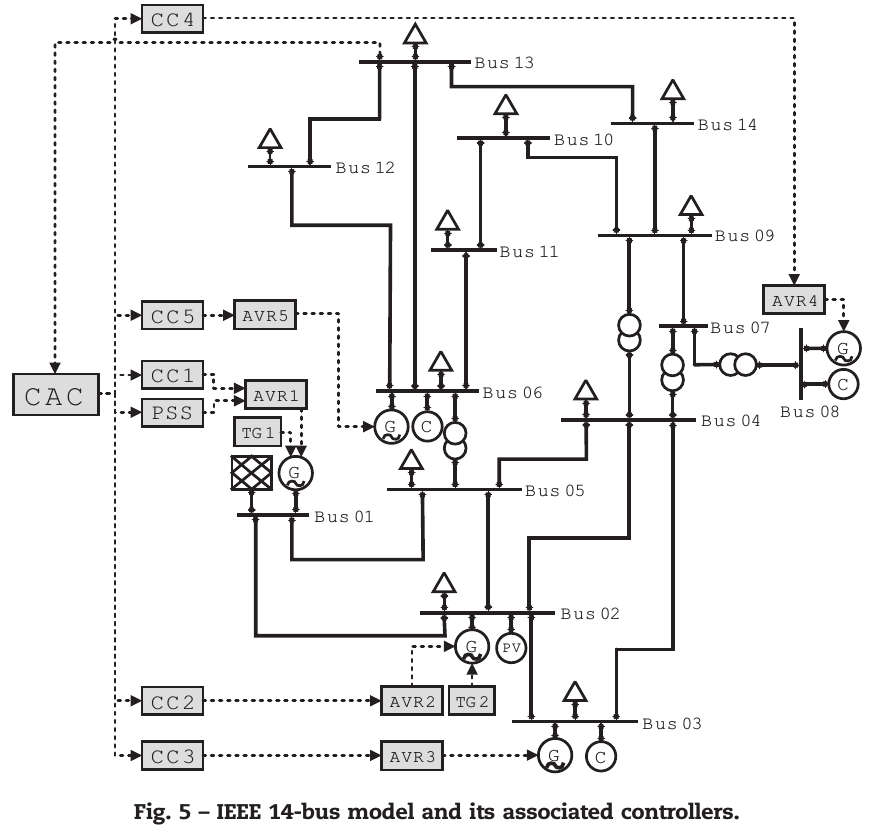
\includegraphics[width=1.0\textwidth]{./images/ieee-14-bus.png}
      % ieee-14-bus.png: 0x0 pixel, 300dpi, 0.00x0.00 cm, bb=
      \label{fig:ieee-14-bus-2}
      \end{figure}
     \end{column}
     \begin{column}{0.45\textwidth}
      \begin{figure}
      \centering
      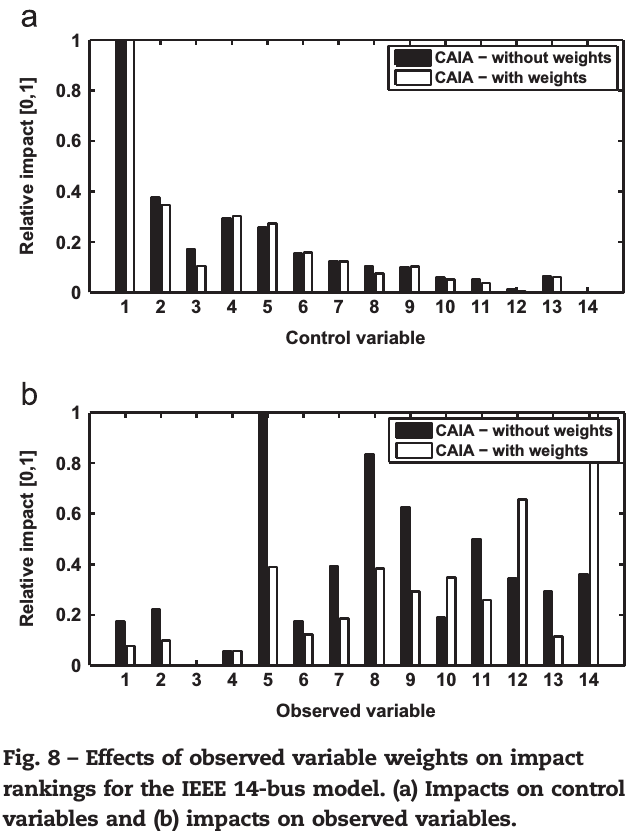
\includegraphics[width=1.0\textwidth]{./images/caia-param-impact.png}
      % caia-param-impact.png: 0x0 pixel, 300dpi, 0.00x0.00 cm, bb=
      \label{fig:caia-param-impact}
      \end{figure}
     \end{column}
    \end{columns}
\end{frame}
\begin{frame}{A system dynamics approach for assessing the impact of cyber attacks on CI (2015)}
    \begin{figure}
    \centering
    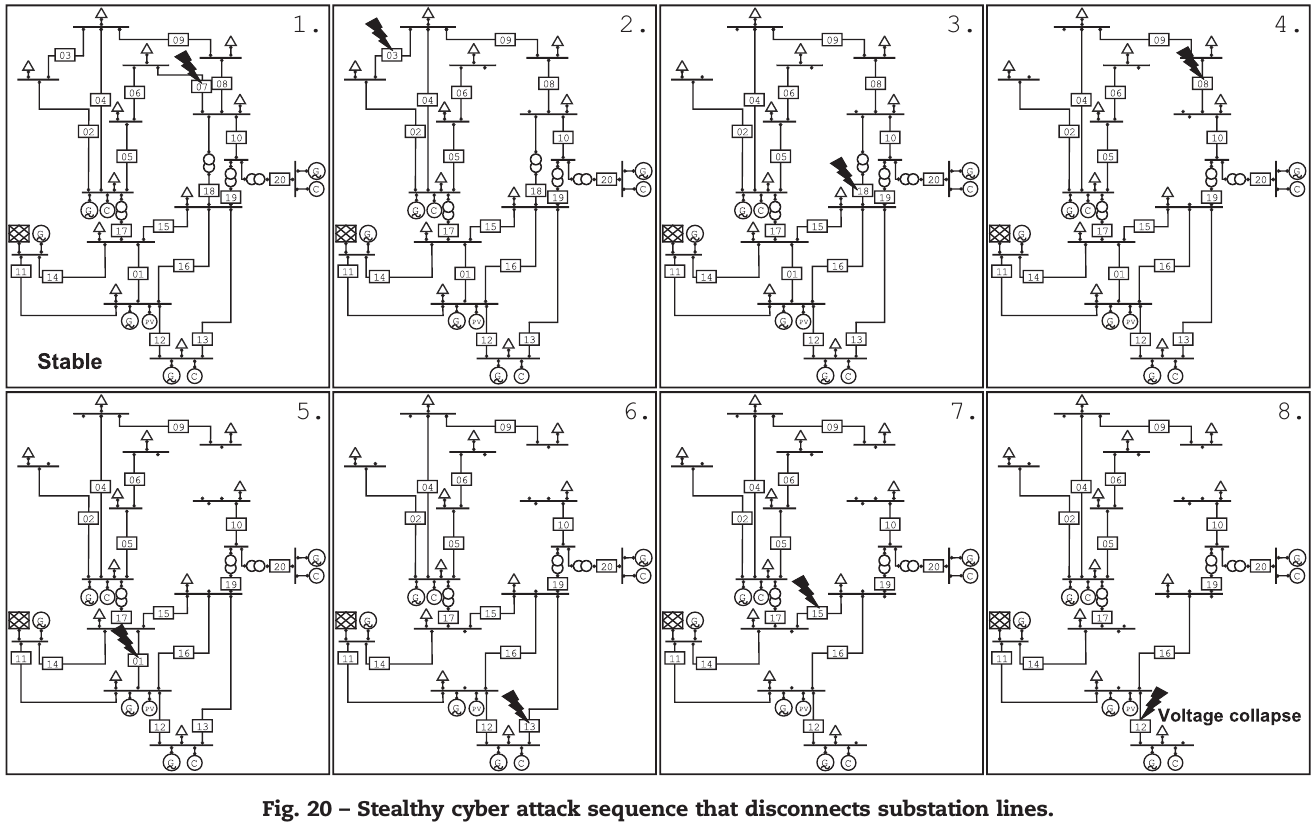
\includegraphics[width=1.0\textwidth]{./images/stealthy-attack-sequence.png}
    % stealthy-attack-sequence.png: 0x0 pixel, 300dpi, 0.00x0.00 cm, bb=
    \label{fig:stealthy-attack-sequence}
    \end{figure}
\end{frame}
\begin{frame}{A system dynamics approach for assessing the impact of cyber attacks on CI (2015)}
    \begin{columns}
     \begin{column}{0.4\textwidth}
      \begin{figure}
      \centering
      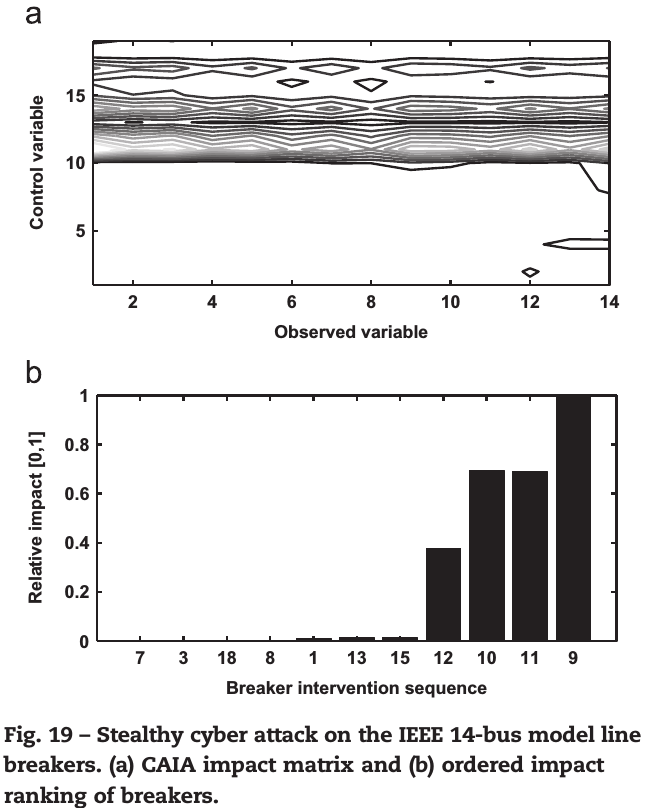
\includegraphics[width=1.0\textwidth]{./images/caia-impact-stealthy.png}
      % caia-impact-stealthy.png: 0x0 pixel, 300dpi, 0.00x0.00 cm, bb=
      \label{fig:ieee-14-bus}
      \end{figure}
     \end{column}
     \begin{column}{0.6\textwidth}
      \begin{figure}
      \centering
      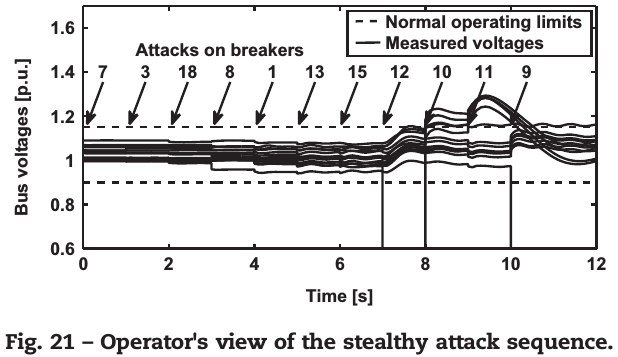
\includegraphics[width=1.0\textwidth]{./images/stealthy-operator-view.png}
      % stealthy-operator-view.png: 0x0 pixel, 300dpi, 0.00x0.00 cm, bb=
      \label{fig:stealthy-operator-view}
      \end{figure}
     \end{column}
    \end{columns}
\end{frame}
\begin{frame}{A system dynamics approach for assessing the impact of cyber attacks on CI (2015)}
    \textbf{Limitations}
    \begin{itemize}
     \item CAIA helps to identify and rank assets given specific interventions (e.g., an attack)
     \item Which interventions are relevant to test (?), and, how to protect the assets after generating the impact matrix (?) are open questions; out of the paper's scope.
     \item Obvious Note: the knowledge of impact matrices would be definitely valuable to attackers(!); as any risk assessment information.
     \item Seems hard to reproduce since no detailed information is given about the simulations; plus, no source code.
    \end{itemize}
\end{frame}
\begin{frame}{Multi-stage Attack Detection and Signature Generation with ICS Honeypots (2016)}
    \textbf{Aim \& Contribution}
    \begin{itemize}
     \item HosTaGe: honeypot for detecting \textbf{multi-stage attacks} in ICS networks.
     \item Honeypot extension with capabilities of ICS protocols, i.e., Modbus, S7, SNMP, HTTP, Telnet, SMB and SMTP.
     \item Basic functions:
     \begin{enumerate}
      \item notify the network administrators;
      \item produce an attack signature;
      \item forward the signature to the internal IDSs.
     \end{enumerate}
    \end{itemize}
\end{frame}
\begin{frame}{Multi-stage Attack Detection and Signature Generation with ICS Honeypots (2016)}
    \textbf{Expermients \& Comparisons}
    \begin{itemize}
     \item HosTaGe was \textbf{compared} with ``CONPOT ICS/SCADA Honeypot''~\footnote{http://conpot.org/}
     \item Criteria:
     \begin{enumerate}
      \item ability to not be evade (i.e., be perceived by attackers);
      \item ability to detect multi-stage attacks;
      \item ability to generate valid signatures for Bro IDS~\footnote{https://www.bro.org/}.
     \end{enumerate}
    \end{itemize}
\end{frame}
\begin{frame}{Multi-stage Attack Detection and Signature Generation with ICS Honeypots (2016)}
    \textbf{Formal Model - Extended Finite State Machine (EFSM)}
    \begin{figure}
    \centering
    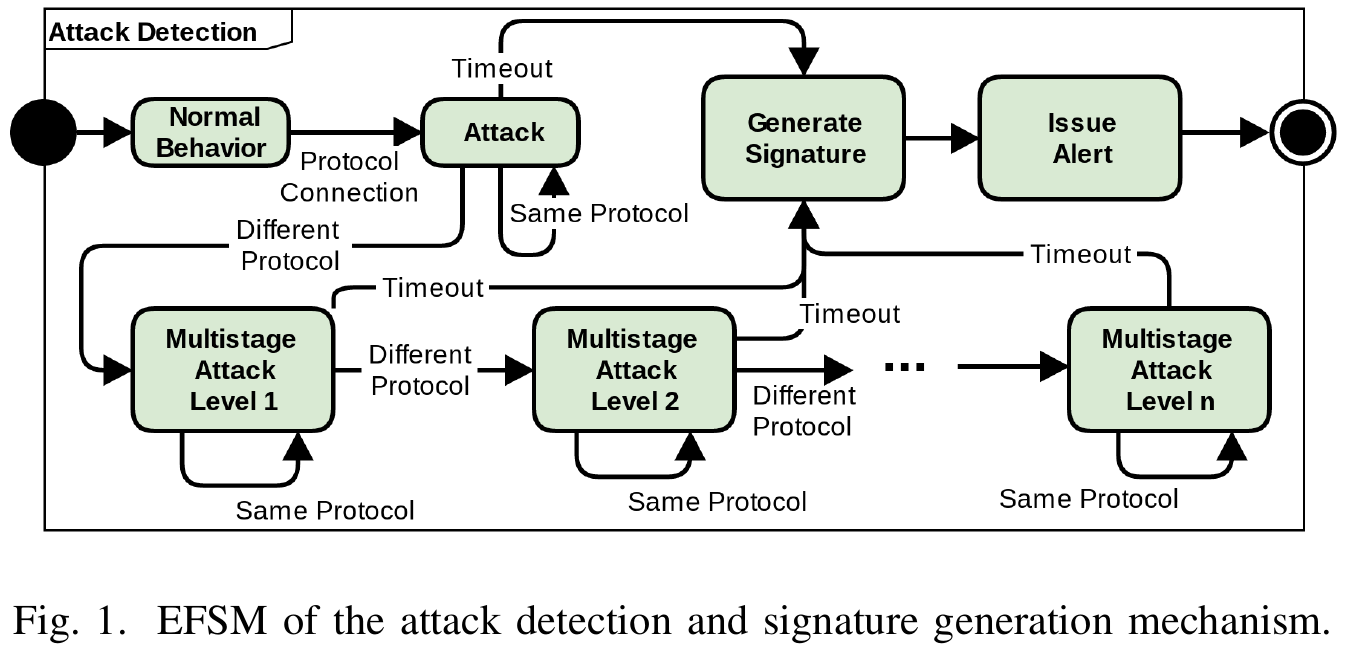
\includegraphics[width=1.0\textwidth]{./images/hostage-efsm.png}
    % hostage-efsm.png: 0x0 pixel, 300dpi, 0.00x0.00 cm, bb=
    \label{fig:hostage-efsm}
    \end{figure}
\end{frame}
\begin{frame}{Multi-stage Attack Detection and Signature Generation with ICS Honeypots (2016)}
    \textbf{Formal Model - Extended Finite State Machine (EFSM)}
    \begin{itemize}
     \item Detection Mechanism
     \begin{enumerate}
      \item Single-Protocol Level Detection (SPLD)
      \item Multi-Stage Level Detection (MSLD)
      \item Payload Level Detection (PLD)
     \end{enumerate}
     \item \textbf{Time window} ($tw$) determines whether an attack should be mapped as SPLD or MSLD
    \end{itemize}
\end{frame}
% \begin{frame}{Multi-stage Attack Detection and Signature Generation with ICS Honeypots (2016)}
%     Example - Detection of Stuxnet
%     \begin{figure}
%     \centering
%     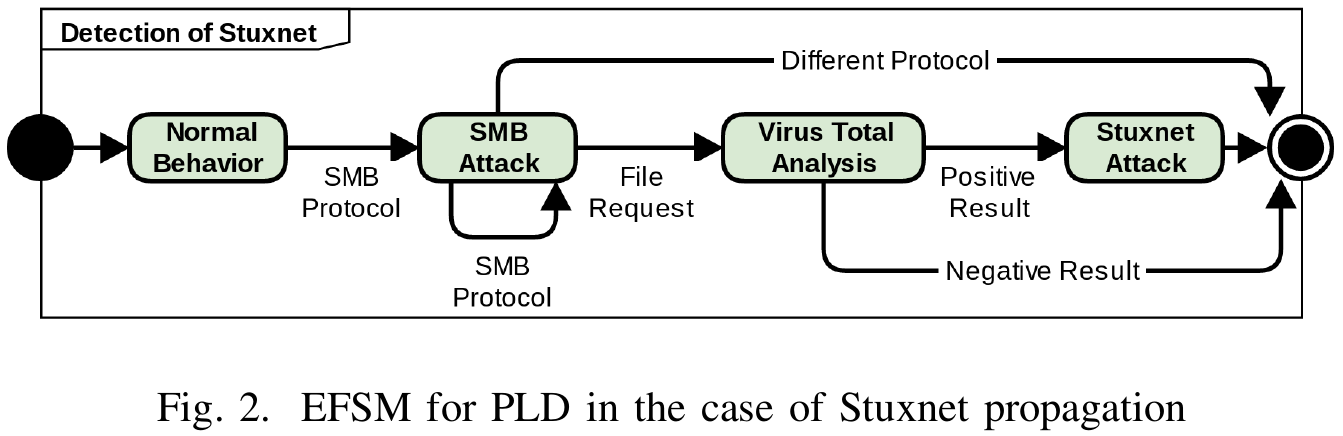
\includegraphics[width=1.0\textwidth]{./images/hostage-stuxnet-detection.png}
%     % hostage-stuxnet-detection.png: 0x0 pixel, 300dpi, 0.00x0.00 cm, bb=
%     \label{fig:hostage-stuxnet-detection}
%     \end{figure}
% \end{frame}
\begin{frame}{Multi-stage Attack Detection and Signature Generation with ICS Honeypots (2016)}
    \textbf{Example - Signature Generation}
    \begin{itemize}
     \item Automatically generate signature for well-known Metasploit script\footnote{No further information given by the authors...} for Modbus services identification.
    \end{itemize}
    \begin{figure}
    \centering
    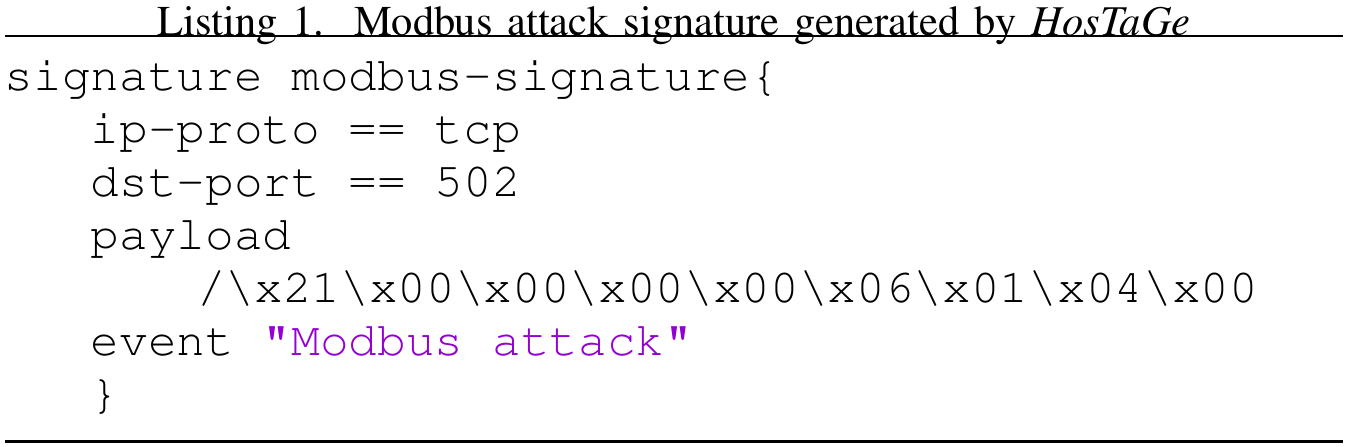
\includegraphics[width=1.0\textwidth]{./images/hostage-signature.png}
    % hostage-signature.png: 0x0 pixel, 300dpi, 0.00x0.00 cm, bb=
    \label{fig:hostage-signature}
    \end{figure}
\end{frame}
\begin{frame}{Multi-stage Attack Detection and Signature Generation with ICS Honeypots (2016)}
    \textbf{Comparison - Honeypot x CONPOT}
    \begin{itemize}
     \item Controlled environment, no firewalls, 8 to 12 weeks, probing by Shodan\footnote{https://www.shodan.io/}.
    \end{itemize}
    \begin{columns}
     \begin{column}{0.55\textwidth}
      \begin{figure}
      \centering
      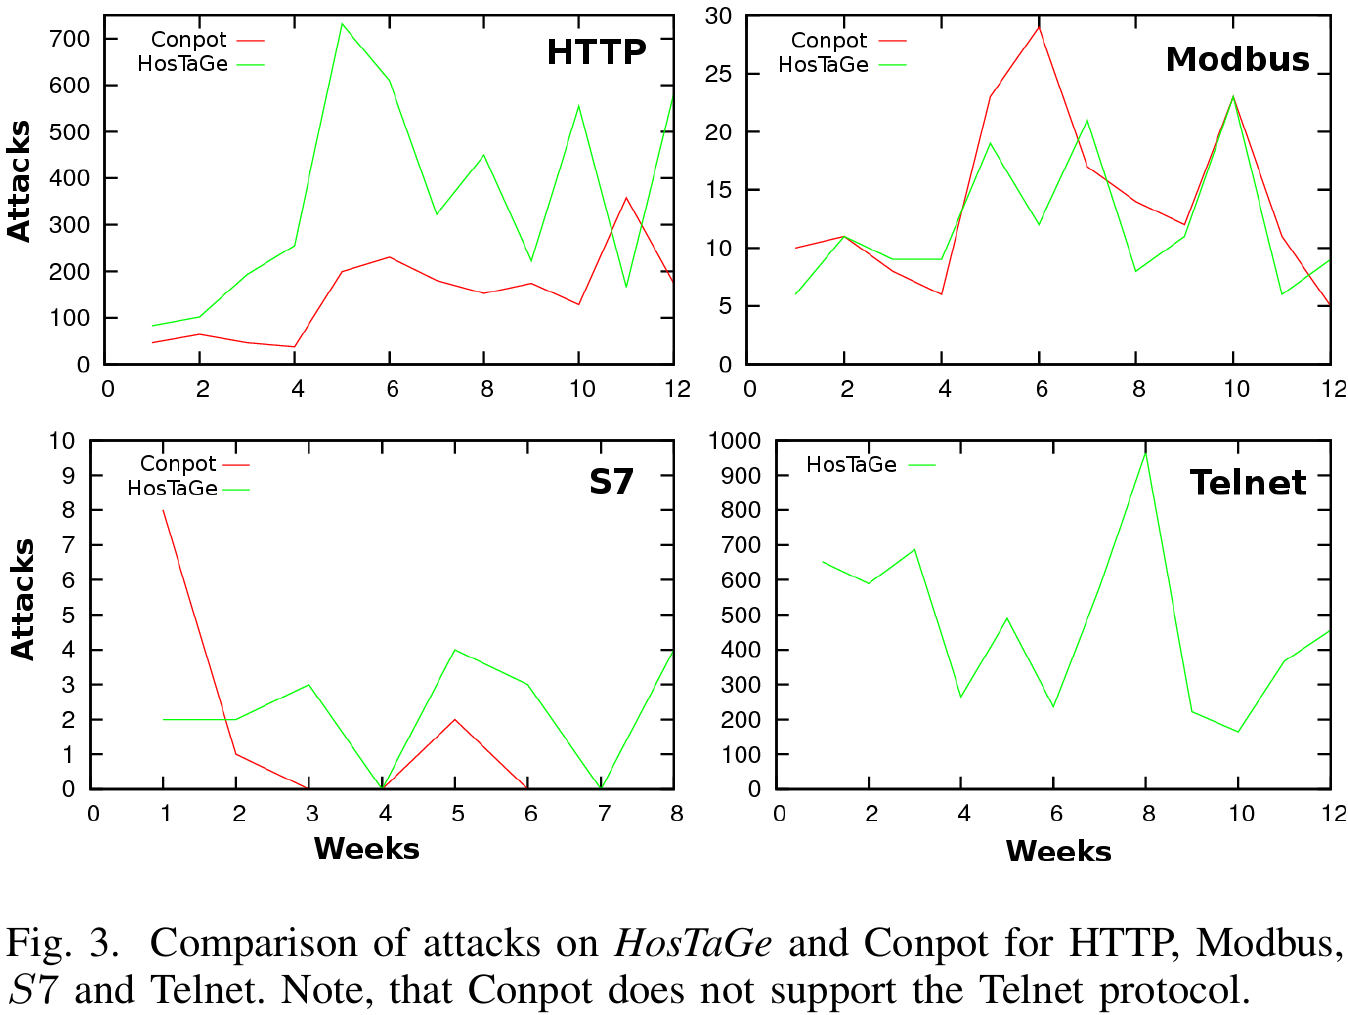
\includegraphics[width=1.0\textwidth]{./images/hostage-conpot-comparison.png}
      % hostage-conpot-comparison.png: 0x0 pixel, 300dpi, 0.00x0.00 cm, bb=
      \label{fig:hostage-conpot-comparison}
      \end{figure}
     \end{column}
     \begin{column}{0.45\textwidth}
      \begin{figure}
      \centering
      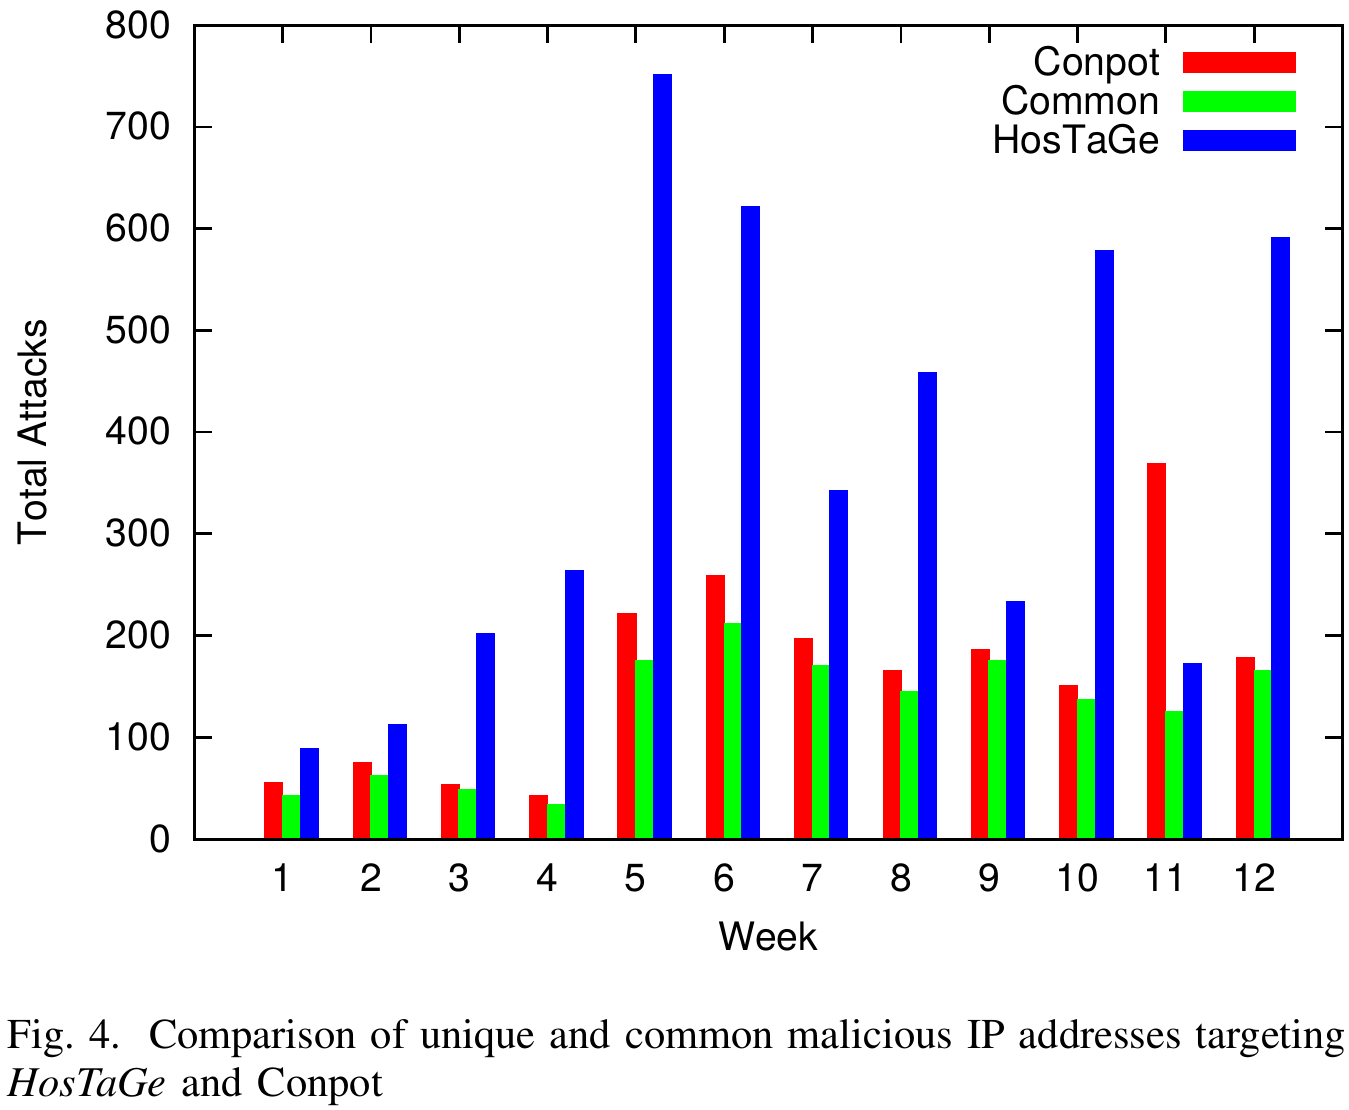
\includegraphics[width=1.0\textwidth]{./images/hostage-ip-sources.png}
      % hostage-ip-sources.png: 0x0 pixel, 300dpi, 0.00x0.00 cm, bb=
      \label{fig:hostage-ip-sources}
      \end{figure}
     \end{column}
    \end{columns}
\end{frame}
\begin{frame}{Multi-stage Attack Detection and Signature Generation with ICS Honeypots (2016)}
    \textbf{Limitations}
    \begin{itemize}
     \item The evaluation of multi-stage signature generation was rather shallow.
     \item Shodan's probes were not explained in details, i.e., how Shodan detect a honeypot?
    \end{itemize}
    More info about HosTaGe can be found at Darmstad's research group website\footnote{https://www.tk.informatik.tu-darmstadt.de/de/research/secure-smart-infrastructures/hostage/}.
\end{frame}

\begin{frame}{Q\&A and Discussions}
      \textbf{Debate Suggestions}
      \begin{itemize}
       \item \textbf{Attacker models} \cite{pasqualetti2013attack,genge2015system} -- strong assumptions; absolute knowledge and control.
       \item \textbf{Study validation} -- enough tests; data sources; experiment description.
       \item \textbf{Reproducibility} -- enough information; open source; plant models.
       \item \textbf{Overall critics} about the papers -- readability; depth; contribution.
      \end{itemize}

\end{frame}

\begin{frame}{Question for paper ``Attack detection and identification in cyberphysical systems (Vasilomanolakis et al, 2013)''}
      \textbf{}
      \begin{enumerate}[(a)]
       \item 
       \item 
       \item 
       \item 
      \end{enumerate}
\end{frame}

\begin{frame}{Question for paper ``Attack detection and identification in cyberphysical systems (Vasilomanolakis et al, 2013)''}
      \textbf{}
      \begin{enumerate}[(a)]
       \item 
       \item 
       \item 
       \item 
      \end{enumerate}
\end{frame}

\begin{frame}{Question for paper ``A system dynamics approach for assessing the impact of cyber attacks on critical infrastructures (Pasqualetti et al, 2015)''.}
      \textbf{Regarding the Cyber Attack Impact Assessment (CAIA) methodology proposed in the paper, which of the following statements is FALSE:}
      \begin{enumerate}[(a)]
       \item CAIA helps system administrators to analyze how cyber attacks affect the normal functioning of physical processes.
       \item The proposed approach computes the covariances of observable variables before and after an specific intervention in control variables.
       \item CAIA methodology is mainly inspired in graph-theoretical and electric centrality metric approaches.
       \item CAIA helps to identify and rank assets in the context of critical infrastructures.
      \end{enumerate}
\end{frame}

\begin{frame}{Question for paper ``A system dynamics approach for assessing the impact of cyber attacks on critical infrastructures (Pasqualetti et al, 2015)''.}
      \textbf{The proposed methodology (CAIA) was validated by various experiments. Which of the following statements is FALSE:}
      \begin{enumerate}[(a)]
       \item The conducted experiments were able to demonstrate CAIA's efficiency, scalability and cross-sector applicability.
       \item Final results demonstrate that CAIA methodology is only suitable for electric grid models, such as IEEE 14-bus and 300-bus.
       \item To demonstrate CAIA's cross-sector applicability, the authors used the Tennessee Eastman chemical plant model.
       \item The authors described how an attacker can use CAIA results to plan and execute a stealthy cyber attack, in which multiple low-impact variables are affected simultaneously to cause severe infrastructure degradation.
      \end{enumerate}
\end{frame}

\begin{frame}{Question for paper ``Multi-stage Attack Detection and Signature Generation with ICS Honeypots (2016)''}
      \textbf{Regarding the concept of honeypot addressed in the paper, which of the following statements is FALSE:}
      \begin{enumerate}[(a)]
       \item Honeypots exhibit a high rate of false positives.
       \item Honeypots are systems whose only value is to be probed, attacked and compromised.
       \item Honeypots are used to attract malicious users and study their activities.
       \item One essential requirement for honeypots is their ability to remain undetected.
      \end{enumerate}
\end{frame}

\begin{frame}{Question for paper ``Multi-stage Attack Detection and Signature Generation with ICS Honeypots (2016)''}
      \textbf{Regarding the comparative study between HosTaGe and Conpot, which of the following statements is FALSE:}
      \begin{enumerate}[(a)]
       \item Overall, HosTage was able to detect more attacks than Conpot.
       \item The analysis of multi-stage attacks was performed only for HosTaGe.
       \item HosTaGe honeypot presented better evasion (ability to remain undetected) capabilities than CONPOT.
       \item Conpot is not an ICS-specific honeypot and therefore it supports a smaller number of protocols.
      \end{enumerate}
\end{frame}

\begin{frame}[allowframebreaks]{References}\tiny{
\def\newblock{}
\bibliographystyle{plain}
\bibliography{./references.bib}}
\end{frame}
\end{document}
